\chapter{Аналитический раздел}
\label{cha:analysis}
%
% % В начале раздела  можно напомнить его цель
%
В данном разделе анализируется предметная область и определяются требования к разрабатываемой системе.

\section{Анализ предметной области}
Подбор респондентов можно разбить на несколько задач: выбор критериев отбора, поиск по внутренней базе компании, поиск в рекрутинговых агентствах, обзвон или рассылка. При этом необходимо учитывать, что для исследований не подходят люди, часто участвующие в подобных мероприятиях. Также нужно обращать внимание на надежность сведений рекрутинговых агентств. В связи с тем, что описанные задачи выполняются разными независимыми компаниями, для решения задачи необходимо организовать распределенную систему, включающую взаимодействие между собой организаций, которым требуются подобные исследования, рекрутинговых агентств и ассоциаций, контролирующих качество услуг последних.

Каждая из систем представляет собой независимый субъект, функционирующий по определенным законам и правилам. Субъекты взаимодействуют между собой по публичным каналам передачи данных (как синхронным, так и асинхронным).

Схема предметной области представлена на рисунке ~\ref{fig:sc-obl}.

\begin{figure}[ht]
  \centering
  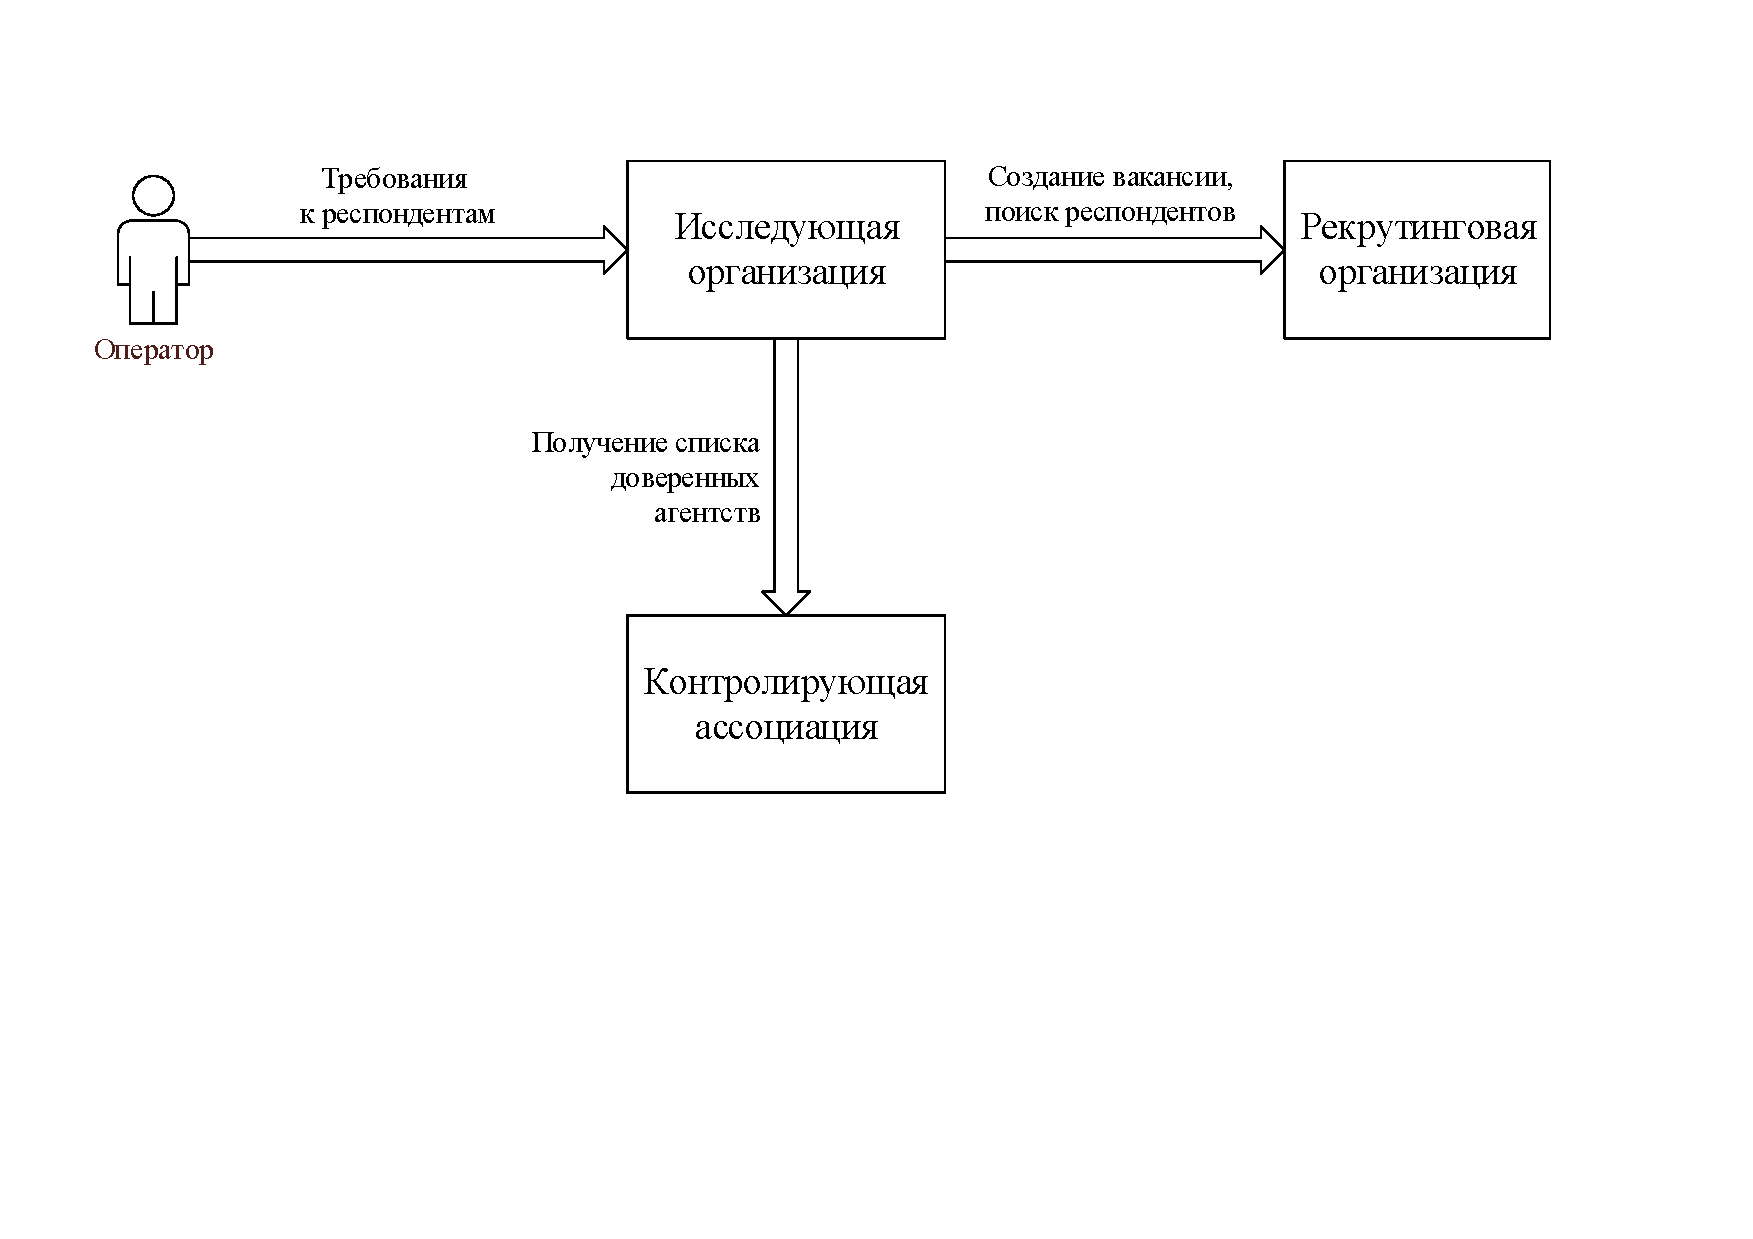
\includegraphics[width=\textwidth]{include/sc-obl.pdf}
  \caption{Схема предметной области}
  \label{fig:sc-obl}
\end{figure}

\section{Описание системы}
Распределенная система состоит из  исследующей организации, рекрутинговых агентств и ассоциаций, контролирующих качество работы последних. В рамках данной работы будут реализованы все эти участники.

На рисунке ~\ref{fig:idef0} изображен процесс функционирования РСОИ. Используются следующие обозначения:
\begin{enumerate}
\item система A — система исследующей организации;
\item система B — система рекрутингового агентства; 
\item система C — система контролирующей ассоциации;
\end{enumerate}

\begin{figure}[ht]
  \centering
  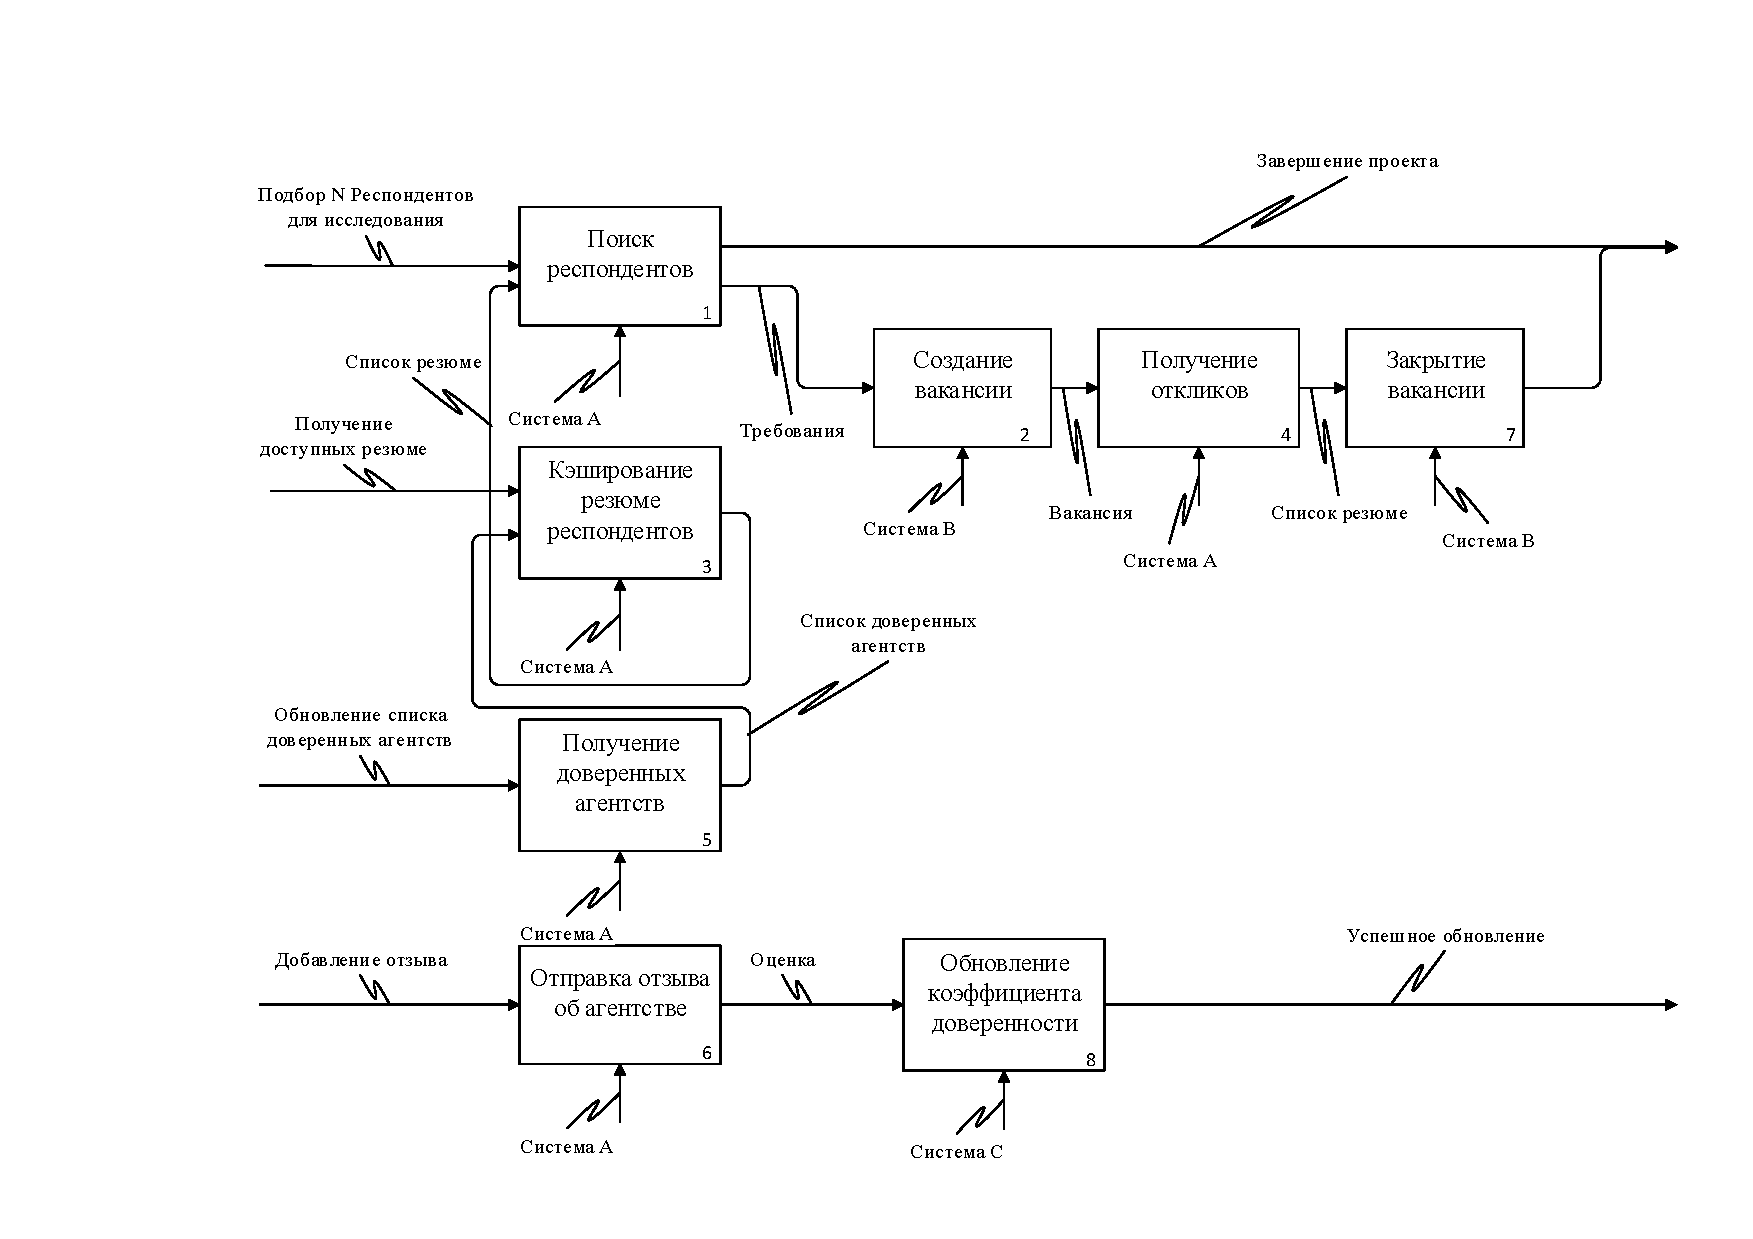
\includegraphics[width=\textwidth]{include/idef0.pdf}
  \caption{Диаграмма функционирования системы}
  \label{fig:idef0}
\end{figure}

Рассмотрим функционирование каждого участника РСОИ.
\begin{enumerate}[1.]
\item Система исследующей организации ~--- предоставляет оператору веб-интерфейс для управления исследованиями, модификации внутренней базы респондентов и создания вакансий для рекрутинговых агентств. Система взаимодействует с рекрутинговыми агентствами и ассоциациями контроля качества услуг. При этом должен быть предусмотрен контроль занятости респондентов, не позволяющий участвовать им одновременно в разных исследованиях. Позволяет оператору изменять и удалять проекты.
\item Система рекрутингового агентства ~--- предоставляет исследующей организации список подходящих респондентов. Множество подходящих людей выбирается автоматически на основе пришедших критерией, участие в конкретном исследовании подтверждается лично респондентом. Система содержит веб-интерфейс пользователя и администратора.
\item Система контролирующей ассоциации ~--- предоставляет исследующей организации данные о надежности рекрутинговых агентств. Собирает данные о работе рекрутинговых агентств (и других организаций, не рассматриваемых в данной работе).
\end{enumerate}

Основной сценарий взаимодействия пользователя с системой представляет собой последовательность следующих действий:
\begin{enumerate}
\itemоператор создает новый проект и определяет требования к респондентам;
\itemсистема выдает набор респондентов из внутренней базы, если этого недостаточно ~--- запрашивается список подходящих людей из рекрутинговых агентств, имеющих высокую оценку качества услуг, там же создается соответствующая вакансия;
\itemсистема рекрутингового агентства подбирает подходящих респондентов и рассылает им уведомления. При подтверждении от респондента его данные начинают выдаваться системе, создавшей вакансию;
\itemоператор договаривается с респондентами, изменяя их статус во внутренней базе;
\itemпо окончании проекта закрываются все вакансии, в рекрутинговые агентства отсылаются данные о реальных участниках исследования;
\itemтакже по окончании проекта оператор может отослать отзыв о качестве услуг рекрутеров;
\itemсистема исследующей организации при получении данных об ухудшении качества работы закрывает все вакансии и прекращает создание новых; при получении данных о новой рекрутинговой компании открывает вакансии там со следующего проекта
\end{enumerate}

В случае закрытия проекта (например, в случае разрыва контракта с клиентом) закрываются все открытые вакансии в рекрутинговых агентствах, а уже отобранным респондентам отсылается письмо с сообщением об этом прискорбном факте.

\section{Требования к системе}
На основе анализа предметной области необходимо сформулировать требования как к всей системе, так и к ее подсистемам.

\subsection{Требования к системе в целом}
\begin{enumerate}
\item Система должна поддерживать добавление новых узлов.
\item Система не должна выходить из строя при выходе из строя одной из подсистем.
\item Обмен информации в системе должен производиться исходя из предположения, что каналы связи небезопасны и ненадежны.
\item Система должна предусматривать восстановление в случае сбоя.
\end{enumerate}

\subsection{Требования к системе исследующей организации}

\textbf{Функциональные требования}
\begin{enumerate}
\item Система должна предоставлять оператору веб-интерфейс.
\item Система должна осуществлять  аутентификацию пользователей по аккаунту в Google Mail.
\item Оператор должен видеть список открытых текущих проектов, информацию об отобранных/требуемых респондентах.
\item Система должна предоставлять оператору возможность изменения внутренней базы респондентов.
\item Система должна предоставлять возможность отправить отзыв о рекрутинговой компании в контролирующую ассоциацию.
\end{enumerate}

\textbf{Входные данные}
\begin{enumerate}
\item Требования к респондентам:
\begin{enumerate}
\item пол;
\item возраст;
\item профессия;
\item доход;
\item прочие особенности (ключевые слова).
\end{enumerate}
\item Количество респондентов, требуемых для исследования:
\end{enumerate}

\textbf{Выходные данные}
\begin{enumerate}
\item список респондентов, отобранных по внутренней базе;
\item список респондентов, присланных из рекрутинговых агентств;
\item коэффициента доверия рекрутинговому агентству, подобравшему респондента
\end{enumerate}

\subsection{Требования к системе рекрутингового агентства}

\textbf{Функциональные требования}
\begin{enumerate}
\item Система должна предоставлять веб-интерфейс администратора и пользователя.
\item Система должна подбирать респондентов по присланным критериям автоматически.
\item Пользователи могут принимать предложения от исследующей организации или отказываться.
\end{enumerate}

\textbf{Входные данные}
\begin{enumerate}
\item описание исследования;
\item требования к респонденту;
\end{enumerate}

\textbf{Выходные данные}
\begin{enumerate}
\item список подходящих респондентов;
\item список согласившихся респондентов.
\end{enumerate}

\subsection{Требования к системе контролирующей ассоциации}

\textbf{Функциональные требования}
\begin{enumerate}
\item Система должна предоставлять веб-интерфейс оператора.
\item Система должна предоставлять список всех контролируемых организаций с коэффициентами доверия.
\item Система должна собирать отзывы о компаниях от других систем или пользователей.
\end{enumerate}

\textbf{Входные данные}
\begin{enumerate}
\item название контролируемой организации;
\item отзыв.
\end{enumerate}

\textbf{Выходные данные}
\begin{enumerate}
\item список контролируемых организаций с оценками надежности;
\end{enumerate}

\section{Сценарии использования системы}
В качестве основных пользователей системы выступают операторы исследующей системы, которые формируют требования к респондентам. В дальнейшем будем называть их просто "оператор". На рисунке ~\ref{fig:usecase} показаны прецеденты исследующей системы. 

\begin{figure}[ht]
  \centering
  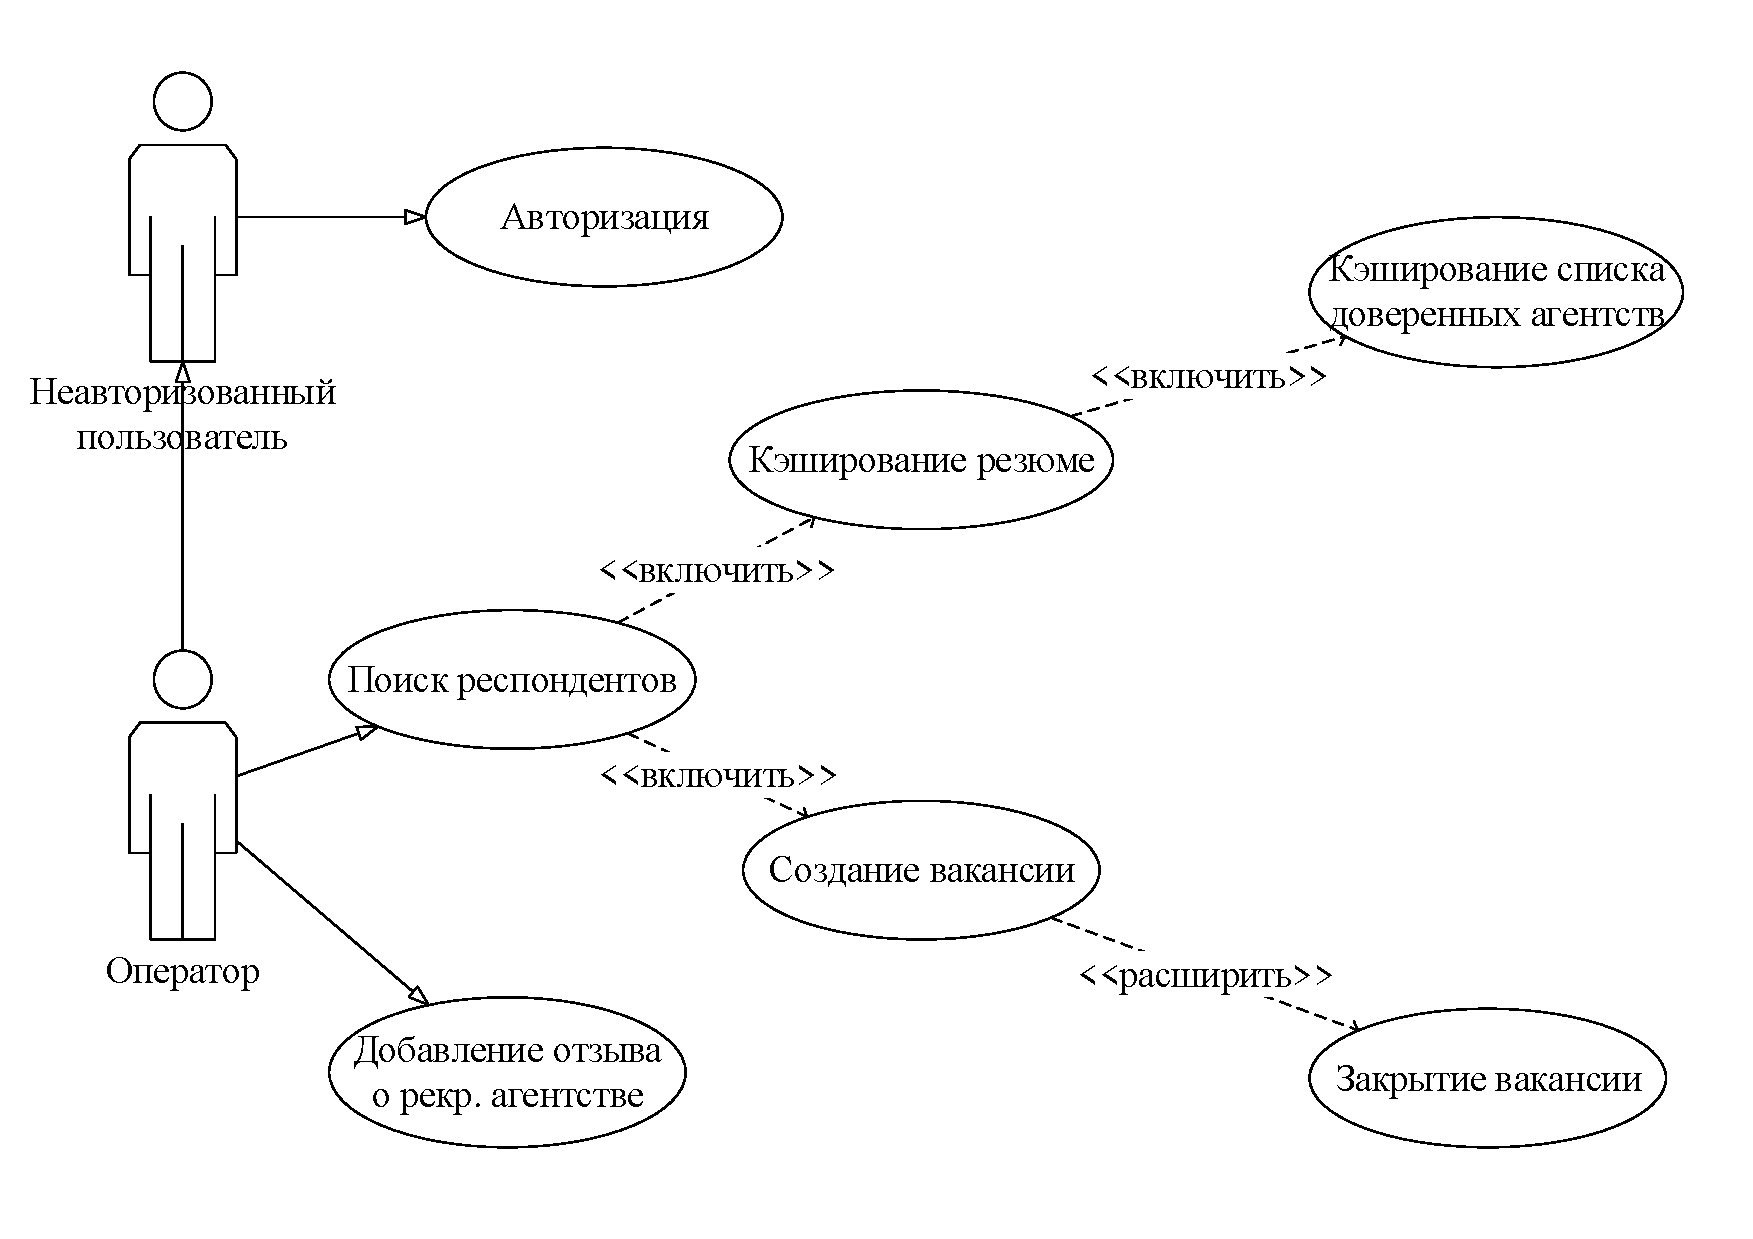
\includegraphics[width=\textwidth]{include/usecase.pdf}
  \caption{Диаграмма прецедентов исследующей системы}
  \label{fig:usecase}
\end{figure}

На стороне контролирующей ассоциации в работе системы участвуют операторы контролирующей системы. Прецеденты для этого участника РСОИ показаны на рисунке ~\ref{fig:usecase1}.

\begin{figure}[ht]
  \centering
  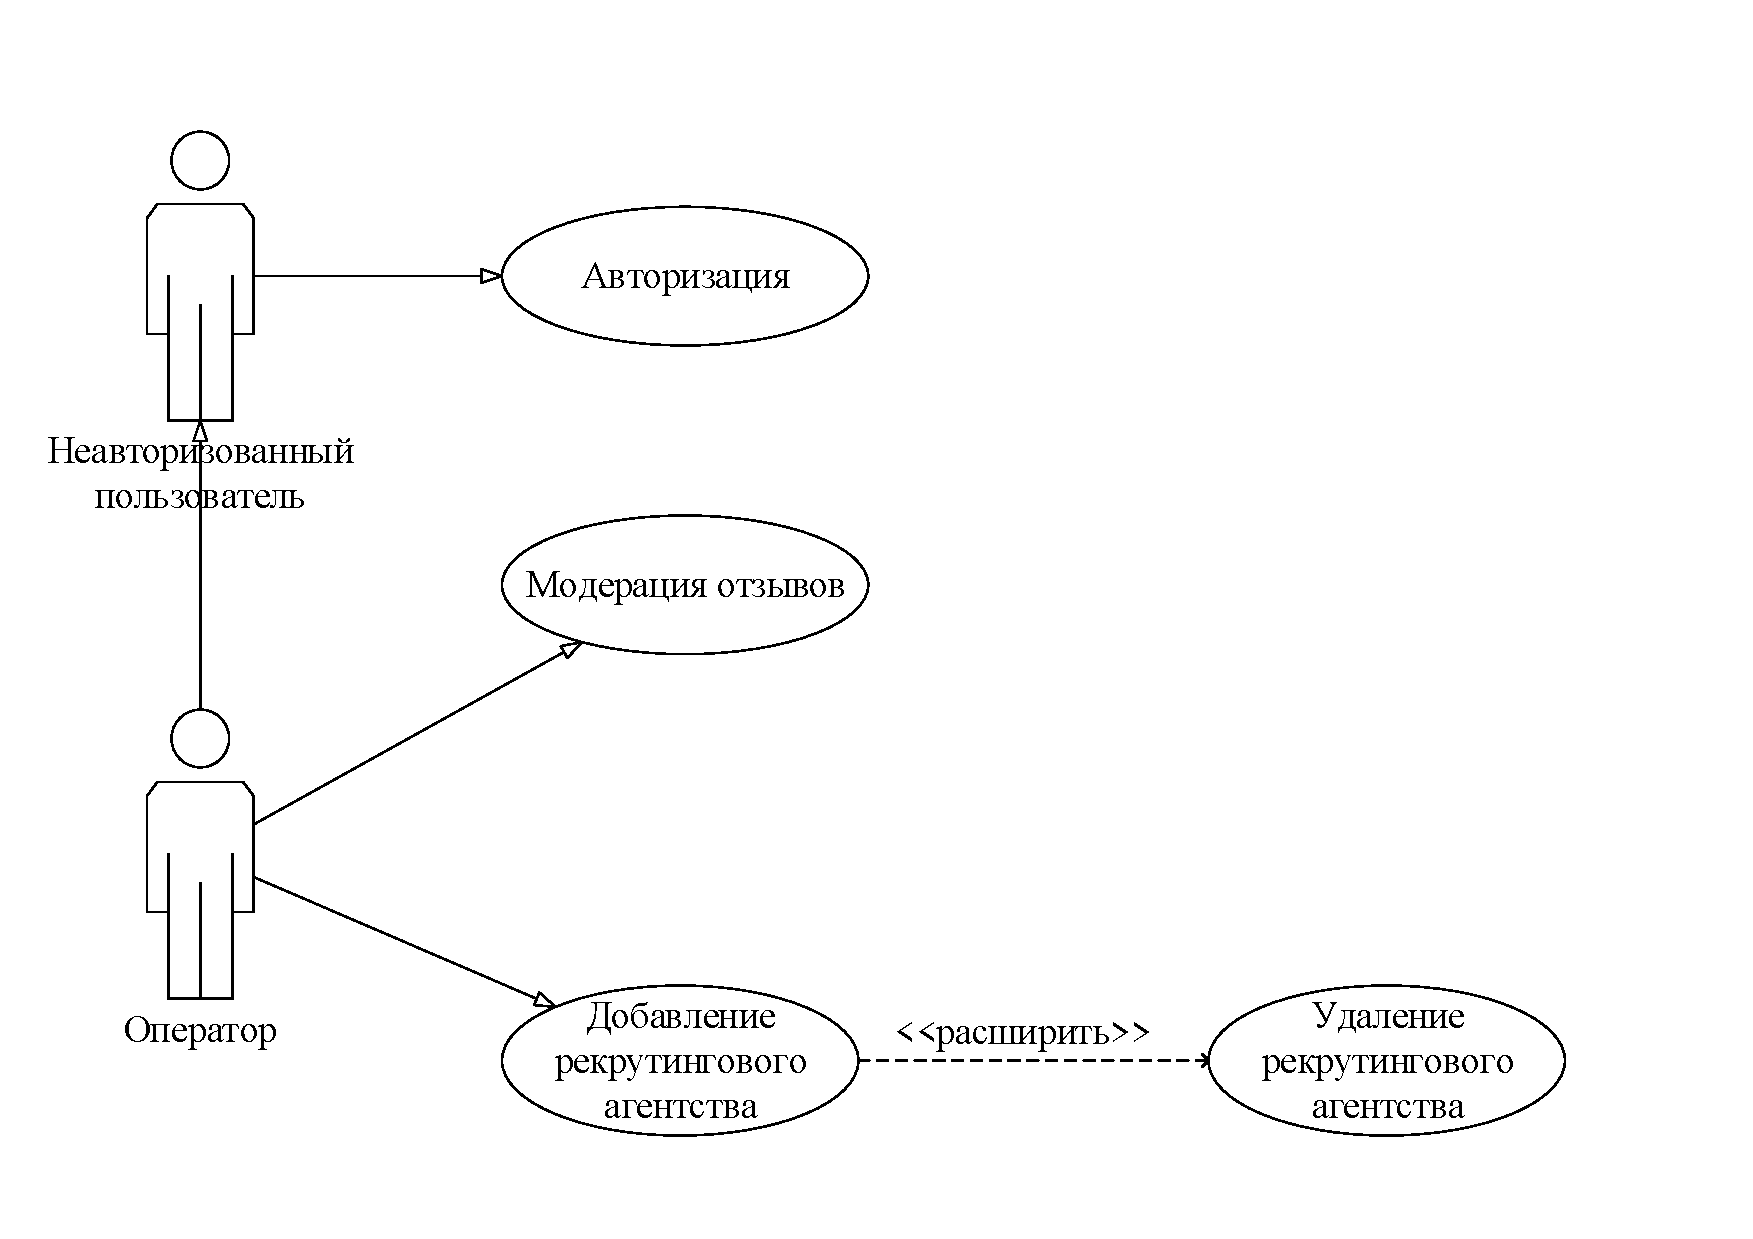
\includegraphics[width=\textwidth]{include/usecase1.pdf}
  \caption{Диаграмма прецедентов контролирующей системы}
  \label{fig:usecase1}
\end{figure}

На стороне рекрутингового агентства в работе участвуют как администраторы, так и пользователи. На рисунке ~\ref{fig:usecase2} отображены прецеденты рекрутинговой системы.

\begin{figure}[ht]
  \centering
  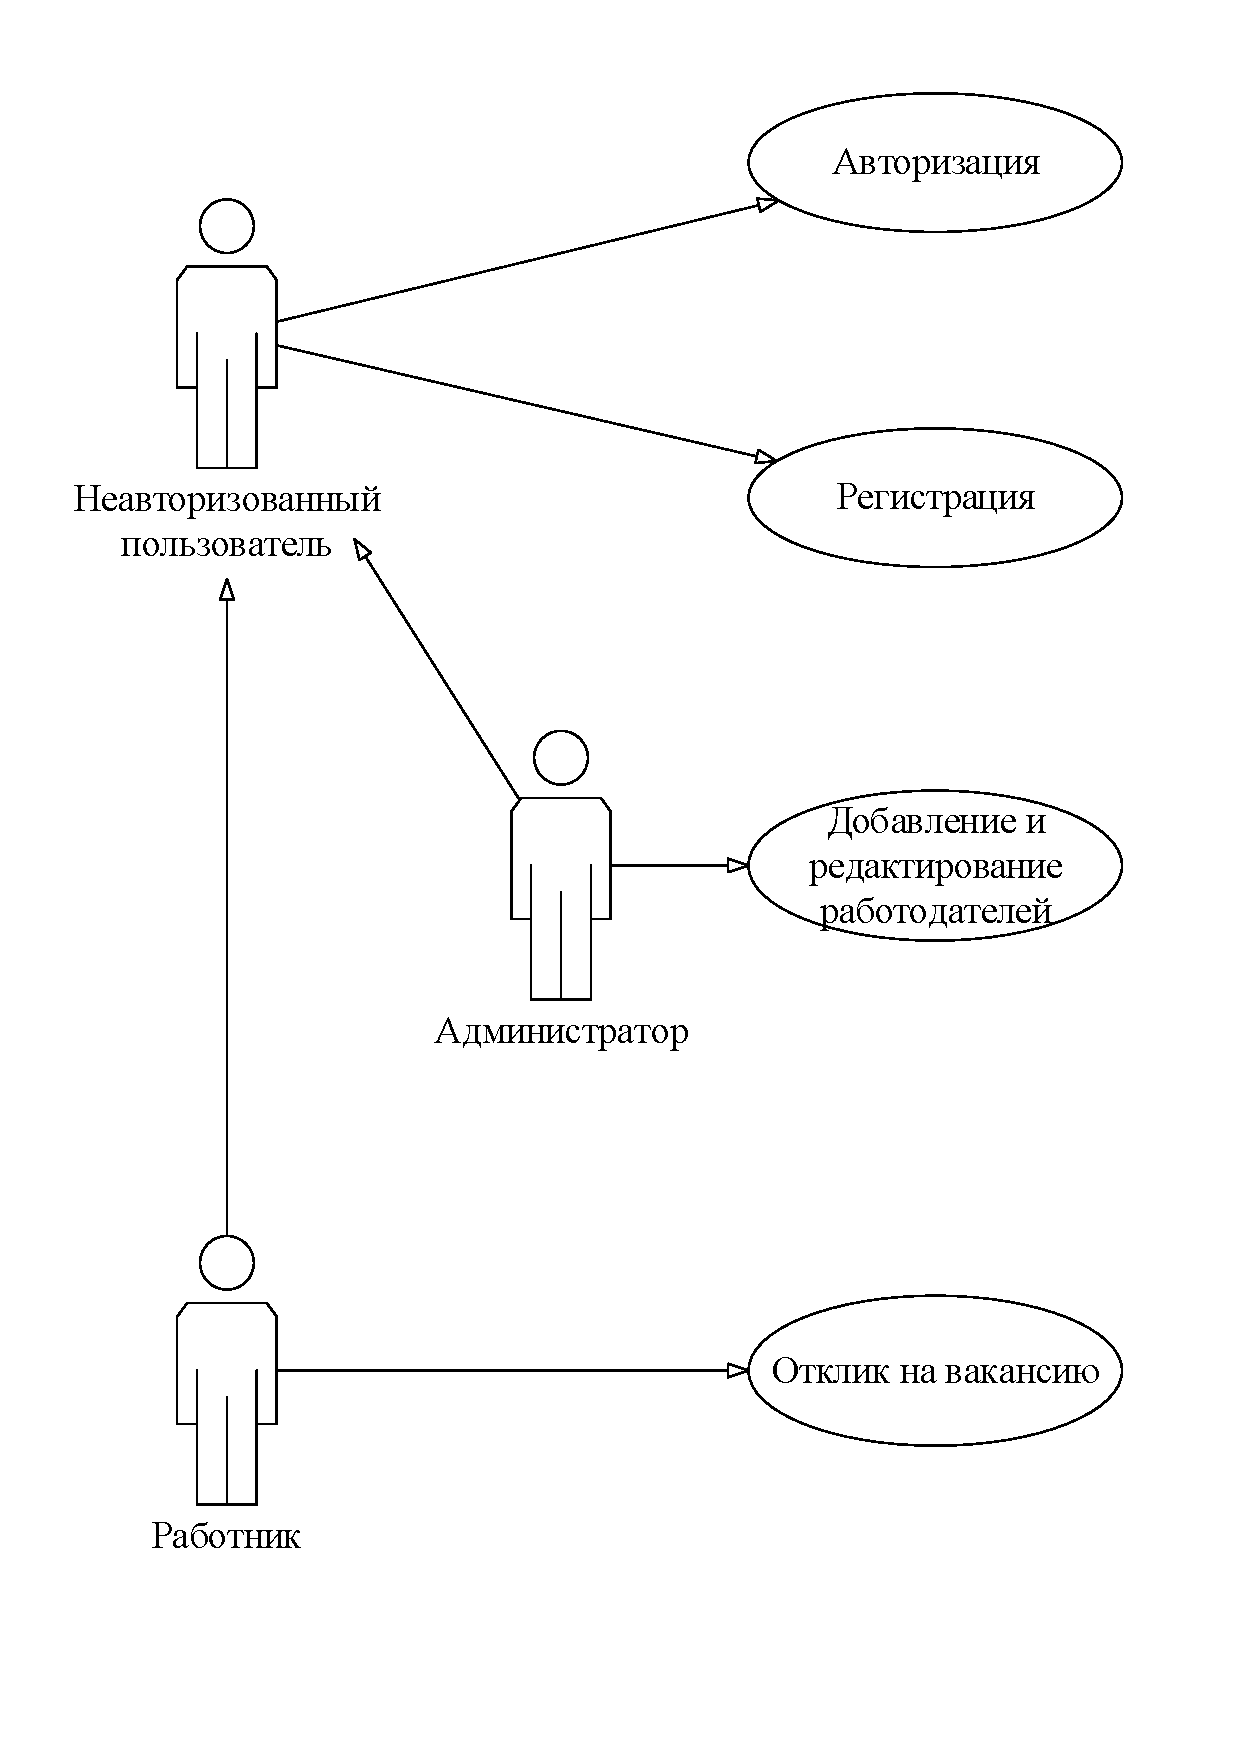
\includegraphics[width=\textwidth]{include/usecase2.pdf}
  \caption{Диаграмма прецедентов рекрутинговой системы}
  \label{fig:usecase2}
\end{figure}

Рассмотрим возможные сценарии:

\textbf{"Вход в систему"}

Краткое описание: оператор входит в систему под своим Google аккаунтом.

\textbf{Сценарий:}\\
Основной поток:
\begin{enumerate}
\item оператор переходит на страницу авторизации исследующей системы. Формируется заявка на OAuth[1].
\item далее он переходит на сайт Google и выбирает почту, с помощью которой он хочет войти;
\item Google  возвращает данные авторизации системе;
\item если данные от Google получены, соответствующий email содержится в базе, а номер заявки на авторизацию существует в системе — оператор переходит на страницу управления проектами.
\end{enumerate}
Альтернативный поток:
\begin{enumerate}
\item оператор выбирает почту на сайте Google, с помощью которой он хочет войти;
\item Google возвращает данные об авторизации системе;
\item если код авторизации отсутствует, либо соответствующий email или номер заявки на авторизацию отсутствует в базе — выводится сообщение об ошибке, оператор остается на странице входа.
\end{enumerate}

\textbf{"Создание проекта"}

Краткое описание: оператор создает новый проект и заполняет требования к респондентам.

\textbf{Сценарий:}\\
Основной поток:
\begin{enumerate}
\item оператор входит в систему;
\item оператор вводит название проекта, требования к респондентам и их количество;
\item система осуществляет поиск по внутренней базе респондентов;
\item в случае, если подходящих респондентов во внутренней базе мало, система создает заявки в доверенных рекрутинговых агентствах;
\item кроме того, осуществляется поиск по кэшированным данным респондентов из рекрутинговых агентств;
\item система выводит результаты поиска и ассоциированные вакансии на экран.
\end{enumerate} 

\textbf{"Отклик на вакансию"}

Краткое описание: респондент из рекрутингового агентства оставил отклик на вакансию.

\textbf{Сценарий:}\\
Основной поток:
\begin{enumerate}
\item система осуществляет опрос рекрутинговых агентств и получает список новых откликов;
\item новые отклики добавляются в список возможных респондентов проекта;
\item оператор обрабатывает новые данные — обзванивает подобранных респондентов или осуществляет рассылку;
\end{enumerate} 

\textbf{"Неуспешное завершение проекта"}

Краткое описание: по неизвестным причинам оператор завершает проект как неуспешный.

\textbf{Сценарий:}\\
Основной поток:
\begin{enumerate}
\item оператор завершает проект как неуспешный;
\item система закрывает все ассоциированные с проектом вакансии;
\item система отсылает письмо всем отобранным респондентам о том, что проект более не существует;
\item система удаляет данные о подходящих и отобранных респондентах для проекта;
\item по желанию оператора оставляется отзыв об использованных рекрутинговых компаниях.
\end{enumerate}

\textbf{"Успешное завершение проекта"}

Краткое описание: исследование было проведено успешно, оператор закрывает проект.

\textbf{Сценарий:}\\
Основной поток:
\begin{enumerate}
\item оператор завершает проект как успешный;
\item система закрывает все ассоциированные с проектом вакансии;
\item система удаляет данные о подходящих и отобранных респондентах для проекта;
\item по желанию оператор может оставить отзыв об использованных рекрутинговых компаниях.
\end{enumerate}

\textbf{"Изменение списка доверенных рекрутинговых агентств"}

Краткое описание: при обновлении данных из контролирующей ассоциации появилось новое доверенное агентство с заданным рейтингом доверия либо уже известное агентство получило рейтинг доверия ниже допустимого.

\textbf{Сценарий:}\\
Основной поток:
\begin{enumerate}
\item система получает список рекрутинговых агентств от контролирующей ассоциации;
\item если используемое рекрутинговое агентство получило рейтинг ниже допустимого - все открытые вакансии и кэшированная база респондентов удаляется, этот участник больше не используется в РСОИ;
\item если появилось новое рекрутинговое агентсво с достаточным рейтингов - для текущих проектов в нем создаются вакансии, обновляется кэшированная база респондентов. Также новый участник используется в РСОИ для последующих проектов.
\end{enumerate}

%%% Local Variables:
%%% mode: latex
%%% TeX-master: "rpz"
%%% End:
